% !TEX encoding = UTF-8
% !TEX TS-program = pdflatex
% !TEX root = ../tesi.tex

%**************************************************************
\chapter{Progettazione e codifica}
\label{cap:progettazione-codifica}
%**************************************************************

\intro{In questo capitolo verranno spiegate le tecnologie utilizzate per lo sviluppo e l'architettura del prodotto software}\\

%**************************************************************
\section{Tecnologie e strumenti}
\label{sec:tecnologie-strumenti}

Di seguito viene data una panoramica delle tecnologie e strumenti utilizzati per lo sviluppo delle maschere e per la collaborazione con i colleghi stagisiti ed il tutor aziendale.

\subsection{Tecnologie}

\subsubsection*{Vue.js}
Vue.js è un framework javascript open source nato nel 2013 che presenta un'architettura adottabile in modo incrementale che si concentra sulla composizione dei componenti, inoltre sono presenti funzionalità avanzate offerte tramite librerie e pacchetti di supporto. I componenti Vue estendono gli elementi HTML di base per incapsulare del codice riutilizzabile quindi a livello generale i componenti sono elementi personalizzati a cui il compilatore Vue associa una particolare funzionalità.\\
Vue utilizza quindi una sintassi basata su HTML e consente di associare il DOM renderizzato ai dati dell'istanza di Vue sottostante. In questo modo i modelli Vue possono essere analizzati da browser e parser HTML conformi alle modifiche ed inoltre con il sistema di reattività Vue è in grado di calcolare il numero minimo di componenti per eseguire nuovamente il rendering applicando la quantità minima di manipolazioni DOM quando cambia lo stato dell'app. Vue presenta un sistema reattivo grazie all'utilizzo di oggetti semplici Javascript ed ad un re-rendering ottimizzato: ogni componente durante il render tiene traccia delle sue dipendenze in modo tale che il sistema sappia quando e di quali componenti deve effettuare nuovamente il render.\\
Un problema che afflige le web application a pagina singola è che quest'ultime forniscono agli utenti la risposta basata solamente sull'URL dal server, di conseguenza l'utilizzo dei segnalibri a determinate schermate e la condivisione dei collegamenti a sezioni specifiche risulta molto difficile se non impossibile. Vue.js per riuscire a risolvere questo problema fornisce un'interfaccia, detta router, che da la possibilità di modificare ciò che viene visualizzato sulla pagina in base all'URL indipendentemente da come esso viene modificato. Infatti Vue.js viene fornito con il pacchetto open source "vue-router" che fornisce un'API per aggiornare l'URL dell'applicazione, supportare la cronologia di navigazione e le reimpostazioni di email e password. Tramite questa tipologia di router i componenti devono essere mappati alla route a cui appartengono per indicare dove deve essere eseguito il loro render.\\
Questo framework implementa il pattern MVVM, acronimo per Model-View-View-Model, una declinazione del più famoso MVC, ovvero Model-View-Controller. I componenti del MVVM sono:
\begin{itemize}
	\item Model (o Modello): l'implementazione del dominio dati come per il classico Modello del pattern MVC;
	\item View (o Vista): il componente grafico renderizzato dall'utente formato da HTML e CSS;
	\item ViewModel (o Vista per il Modello): il collante tra gli altri due componenti, esso fornisce alla View i dati in formato consono alla rappresentazione ed il comportamento di alcuni elementi dinamici.
\end{itemize}

\subsubsection*{Vuetify}
Vuetify è un framework UI completo costruito su Vue.js nel 2014 ed il suo obiettivo è fornire agli sviluppatori gli strumenti per poter creare esperienze utente ricche e coinvolgenti. A differenza di altri framework Vuetify è progettato da zero in modo tale da renderlo facile da imparare ed essere gratificante da padroneggiare con centinaia di componenti realizzate dalle specifiche di Material Design.\\
Un pregio di questo framework è che adotta un approccio al mobile, questo significa che la web application sviluppata tramite esso sarà pienamente utilizzabile immediatamente su un tablet, un telefono ed un computer. Inoltre è un framework in sviluppo attivo che viene aggiornato settimanalmente rispondendo ai problemi e relativi report della community. Un altro pregio è, come si può vedere nell'immagine sottostante, il gran numero di funzionalità che possiede Vuetify in confronto agli altri framework di Vue.
\begin{figure}[H]
	\begin{center}
		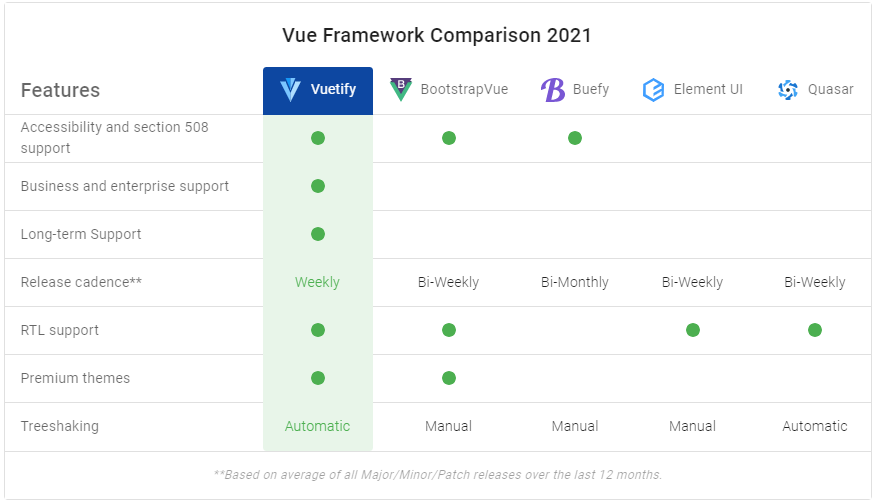
\includegraphics[width=1\columnwidth]{vuetify.png}
		\caption{Funzionalità di Vuetify}
	\end{center}
\end{figure}

\subsection{Strumenti}

\subsubsection{Github}

Github è un servizio fondato nel 2008 di hosting per progetti software ed è un'implementazione dello strumenti di controllo versione distribuito Git.

\subsubsection{Figma}

Figma è uno strumento nato nel 2016 rivolto ai web designer che hanno bisogno di un tool per la progettazione di interfacce. I vantaggi offerti da questo strumento sono i seguenti:
\begin{itemize}
	\item accessibilità multipiattaforma
	\item sistema di collaborazione in real-time
	\item utilizzo degli strumenti responsive oriented per una progettazione ottimale
	\item lavora in vettoriale
\end{itemize}
Grazie a questo strumento io e gli altri stagisti legati all'ambito front end abbiamo potuto creare dei prototipi delle maschere che avremmo dovuto sviluppare.

\subsubsection{Stoplight}

\subsubsection{Visual Studio Code}

%**************************************************************
\section{Ciclo di vita del software}
\label{sec:ciclo-vita-software}

%**************************************************************
\section{Progettazione}
\label{sec:progettazione}

\subsubsection{Namespace 1} %**************************
Descrizione namespace 1.

\begin{namespacedesc}
    \classdesc{Classe 1}{Descrizione classe 1}
    \classdesc{Classe 2}{Descrizione classe 2}
\end{namespacedesc}


%**************************************************************
\section{Design Pattern utilizzati}

%**************************************************************
\section{Codifica}
